\documentclass[BTech]{iitmdiss}

\usepackage{times}
\usepackage{epsf}
\usepackage{threeparttable}
\usepackage{setspace}
\usepackage{amsmath}
\usepackage{amsthm}
\usepackage{txfonts,pxfonts,amsfonts}
\usepackage{epsfig}
\usepackage{caption}
\usepackage{subcaption}
\usepackage{graphicx}
% \usepackage[square]{natbib}
\usepackage[square,numbers, sort]{natbib}
% \usepackage[square,numbers,sort]{natbib}
\usepackage{hyperref} % hyperlinks for references.
\usepackage{algorithm}
\usepackage{algpseudocode}
\usepackage{listings}
\usepackage{color}
\usepackage{color}
\usepackage{tcolorbox}
\usepackage{array}
\usepackage{booktabs}
\usepackage{adjustbox}
\usepackage{dirtytalk} %!!!
\usepackage[T1]{fontenc}
\usepackage{charter}
% \usepackage[expert]{mathdesign}
\usepackage{cleveref}

\definecolor{mygreen}{rgb}{0,0.6,0}
\definecolor{mygray}{rgb}{0.5,0.5,0.5}
\definecolor{mymauve}{rgb}{0.58,0,0.82}

\lstset{ 
  backgroundcolor=\color{white},   % choose the background color; you must add \usepackage{color} or \usepackage{xcolor}; should come as last argument
  basicstyle=\footnotesize\ttfamily,        % the size of the fonts that are used for the code
  breakatwhitespace=false,         % sets if automatic breaks should only happen at whitespace
  breaklines=true,                 % sets automatic line breaking
  captionpos=b,                    % sets the caption-position to bottom
  commentstyle=\color{mygreen},    % comment style
  deletekeywords={...},            % if you want to delete keywords from the given language
  escapeinside={\%*}{*)},          % if you want to add LaTeX within your code
  extendedchars=true,              % lets you use non-ASCII characters; for 8-bits encodings only, does not work with UTF-8
  firstnumber=1,                   % start line enumeration with line 1000
  frame=single,	                   % adds a frame around the code
  keepspaces=true,                 % keeps spaces in text, useful for keeping indentation of code (possibly needs columns=flexible)
  keywordstyle=\color{blue},       % keyword style
  language=C++,                    % the language of the code
  morekeywords={__global__, __shared__, __device__, __host__, __syncthreads},  % if you want to add more keywords to the set
  numbers=left,                    % where to put the line-numbers; possible values are (none, left, right)
  numbersep=5pt,                   % how far the line-numbers are from the code
  numberstyle=\tiny\color{mygray}, % the style that is used for the line-numbers
  rulecolor=\color{black},         % if not set, the frame-color may be changed on line-breaks within not-black text (e.g. comments (green here))
  showspaces=false,                % show spaces everywhere adding particular underscores; it overrides 'showstringspaces'
  showstringspaces=false,          % underline spaces within strings only
  showtabs=false,                  % show tabs within strings adding particular underscores
  stepnumber=1,                    % the step between two line-numbers. If it's 1, each line will be numbered
  stringstyle=\color{mymauve},     % string literal style
  tabsize=2,	                   % sets default tabsize to 2 spaces
  title=\lstname                   % show the filename of files included with \lstinputlisting; also try caption instead of title
}

% Strut macros for skipping spaces above and below text in tables.
\def\abovestrut#1{\rule[0in]{0in}{#1}\ignorespaces}
\def\belowstrut#1{\rule[-#1]{0in}{#1}\ignorespaces}

\def\abovespace{\abovestrut{0.20in }}
\def\aroundspace{\abovestrut{0.20in}\belowstrut{0.10in}}
\def\belowspace{\belowstrut{0.10in}}

\begin{document}
\bibliographystyle{iitm}

% Title page
\title{A GPU based model for Genetic Programming}
\author{Vimarsh Sathia}
\date{June 2021}
\department{COMPUTER SCIENCE AND ENGINEERING}

%\nocite{*}
\begin{singlespace}
\maketitle
\end{singlespace}

% Certificate
\certificate

\vspace*{0.5in}

\noindent This is to certify that the thesis entitled {\bf Implementing Genetic Programming on GPUs}, 
submitted by {\bf Vimarsh Sathia}, to the Indian Institute of Technology, 
Madras, for the award of the degree of {\bf Bachelor of Technology}, 
is a bona fide record of the research work carried out by him under my
supervision. The contents of this thesis, in full or in parts, have not been
submitted to any other Institute or University for the award of any degree or
diploma.

\vspace*{1.4in}
\hspace*{-0.25in}
\begin{singlespacing}
	\hspace*{-0.25in}
	\parbox{2.5in}{
		\noindent {\bf Prof. Rupesh Nasre} \\
		\noindent Research Guide \\ 
		\noindent Professor \\
		\noindent Dept. of CSE\\
		\noindent IIT Madras, 600036 \\
	} 
	\hspace*{1.0in} 
	%\parbox{2.5in}{
	%\noindent {\bf Prof.~S.~C.~Rajan} \\
	%\noindent Research Guide \\ 
	%\noindent Assistant Professor \\
	%\noindent Dept.  of  Aerospace Engineering\\
	%\noindent IIT-Madras, 600 036 \\
	%}  
\end{singlespacing}
\vspace*{0.25in}
\noindent Place: Chennai\\
Date: \today

% Acknowledgements
\acknowledgements

The completion of this thesis would not have been possible without support and assistance from a number of people. 

I would first and foremost like to thank Prof.~Rupesh Nasre for giving me the opportunity to be able to work on this project. Starting from introducing me to Nvidia's open source project maintainers all the way to reviewing the contents of this thesis, he has been very supportive in all the steps of this project. I am deeply grateful for his guidance and help in this project. 

On Nvidia's side, I would like to thank Mr.~Venkatramana G. and Mr.~Thejaswi N. S. for patiently guiding me through the process of merging my code with the \texttt{cuML} library. The bi-weekly discussions held with them about the code gave me valuable insights into the process of open source development, and made me realize the importance of continuous feedback in long-term projects. 

Finally, I would like to thank all my friends from college, who have made the past $4$ years memorable, and my family for their unconditional love and support.

% Abstract
\abstract

\noindent KEYWORDS: \hspace*{0.5em} 
\parbox[t]{4.4in}{  
  Genetic Programming;
	Symbolic Regression; 
  CUDA;
  GPGPU programming; 
  Stack-based virtual machines; 
}

\vspace*{24pt}

\noindent Genetic Programming(GP) is a domain-independent technique for evolving computer programs on the principles of genetics and natural selection. In the context of machine learning, it is one example of an evolutionary algorithm, which iteratively finds solutions to optimization problems through fitness functions and repeated evolution. As such, GP has several inherently parallel steps, making it an ideal candidate for GPU based parallelization. 

In this thesis, we describe the implementation details of a parallel stack-based GP algorithm, to be used for the purpose of symbolic regression and transformation. To achieve higher performance and scalability, we parallelize the selection and evaluation step of the generational GP algorithm. 
For the selection step, tournament selections are vectorized across the entire population using CUDA kernels. 
Parallel evaluation is achieved by representing candidate expression ASTs using prefix lists, which are then evaluated using a fixed length stack in GPU memory.
We also provide fully vectorized kernels to enable fast fitness computations for $6$ common loss functions. For mutations, a hoisted version of the crossover operation is also presented as a depth-conscious alternative to the traditional crossover operation.

We then run benchmarks on synthetic datasets (ranging in size from $4096$ to $4$ million rows) for the Pagie Polynomial, profiling execution times for our algorithm and other standard GP libraries. For our implementation, we also study the effect of the number of generations and dataset sizes on the best fitness value achieved using the Root Mean Square(RMS) metric. Finally, we also study the effect of increasing dataset sizes on walltimes taken by the evaluation step, in an effort to identify bottlenecks in our algorithm.

Using Nvidia Turing GeForce GTX 1650 GPUs, average speedups of upto $27$x were observed on the performance benchmarks of our algorithm against gplearn, a CPU-only symbolic regression library. Using a $4$ million row dataset, our algorithm can fit a symbolic regressor with $50$ expression trees evolved for $50$ generations in less than $10$ seconds. 

% JoJo - Dammit! Now that it has come to this, it is time to use the secret Joestar technique! 
% Dio - NANI?? What is this? Did the Joestars develop some secret powers while I was away for the past 100 years? 
% JoJo - Nigerundayo, Smokey!!!

% Table of contents
\begin{singlespace}
\tableofcontents
\thispagestyle{empty}

\listoftables
\addcontentsline{toc}{chapter}{LIST OF TABLES}
\listoffigures
\addcontentsline{toc}{chapter}{LIST OF FIGURES}
\end{singlespace}

\abbreviations
 
\noindent 
\begin{tabbing}
xxxxxxxxxxx \= xxxxxxxxxxxxxxxxxxxxxxxxxxxxxxxxxxxxxxxxxxxxxxxx \kill
\textbf{GP}   \> Genetic Programming \\
\textbf{EC}   \> Evolutionary Computing \\
\textbf{EA}   \> Evolutionary Algorithm \\
\textbf{GPU}  \> Graphics Processing Unit \\
% \textbf{CUDA} \> Compute Unified Device Architecture \\
% \textbf{SIMD} \> Single Instruction Multiple Data \\
% \textbf{AoS} \> Array of Structures \\
% \textbf{DAG} \> Directed Acyclic Graph
\end{tabbing}
% \pagebreak
% \chapter*{\centerline{NOTATION}}
\addcontentsline{toc}{chapter}{NOTATION}
 
\begin{singlespace}
  \begin{tabbing}
    xxxxxxxxxxx \= xxxxxxxxxxxxxxxxxxxxxxxxxxxxxxxxxxxxxxxxxxxxxxxx \kill
    \textbf{$r$}  \> Radius, $m$ \\
    \textbf{$\alpha$}  \> Angle of thesis in degrees \\
    \textbf{$\beta$}   \> Flight path in degrees \\
  \end{tabbing}
\end{singlespace}
 
\pagebreak
\clearpage

%The main text will follow from this point so set the page numbering
%to arabic from here on.
\pagenumbering{arabic}

% Chapters start here
\chapter{INTRODUCTION} \label{chap:intro}
In recent years, there has been a widespread increase in the use of GPUs in the field of machine learning and deep learning, because of their ability to massively speedup the training of models. This is mainly due to the large parallel processing ability of GPUs, which can process multiple inputs using SIMD intrinsics. Genetic Programming(GP) is a class of machine algorithms with several inherent parallel steps. As such, it is an ideal domain for GPU based parallelization. 

\section{The Problem}
\label{intro:problem}
Genetic  Programming is a technique which involves evolving a set of programs based on the principles of genetics and natural selection. It is a generalized heuristic search technique, which searches for the best program optimizing a given fitness function. 
As such it has applications ranging from machine learning to code synthesis\citep{Koza92}. It also supports a meta-evolutionary framework, where a GP system itself can be evolved using GP\citep{schaul2010metalearning}.

However, in practice, it is difficult to scale GP algorithms. Fitness evaluation of candidate programs in GP algorithms is a well-known bottleneck and there are multiple previous attempts to overcome this problem - either through parallelization of the evaluation step\citep{10.1007/978-3-540-71605-1_9,baeta2021tensorgp,DEAP_JMLR2012,gplearn,staats2017tensorflow}, or by eliminating the need for fitness computations itself through careful initialization and controlled evolution\citep{biles2001autonomous}.

\section{Our Contributions}
\label{intro:contrib} 
In this thesis, we provide details about a parallelized version of the generational GP algorithm to solve the problems of Symbolic Regression and Transformation. We use a stack-based GP algorithm for simplified program evaluation(inspired by \citep{perkis}). Our algorithm can also be used to train symbolic binary-classifiers, where the classifier's output corresponds to the estimated equation of the decision boundary. 

Our main contributions are listed below:
\begin{itemize}
  \item We parallelize the selection and evaluation step of the generational GP algorithm, by conducting parallel tournaments and vectorizing evaluation across the dataset as well as the candidate population. 
  \item We introduce a prefix-tree based Array of Structures (AoS) representation for candidate programs, along with a CUDA kernel to execute all programs on a dataset using a thread-local stack optimized for memory access. 
  \item We also provide a new method to perform tournaments for program selection in parallel using random numbers generated inside the GPU. 
  \item Execution time benchmarks for program evaluation for our algorithm are then provided. The same benchmarks are also run on other standard libraries like gplearn\citep{gplearn} and TensorGP\citep{baeta2021tensorgp}, for comparing training speeds. We then study the effect of population size and dataset size on the final time taken for training. We also conduct a brief analysis of the results of executing our algorithm on synthetic datasets for the Pagie Polynomial\cite{Pagie1997}.
\end{itemize}

% YOU FELL FOR IT FOOL! THUNDER CROSS SPLIT ATTACK
The code for our algorithm is a part of the cuML library\citep{raschka2020machine}, a library intended to be a GPU accelerated version of the scikit-learn
library\citep{scikit-learn}. The library is a part of the RAPIDS suite of open source libraries maintained by Nvidia Corporation.

\section{Outline}
\label{intro:outline}

The rest of this thesis is structured in the following way. 
\begin{itemize}
  \item \Cref{chap:bgrw} introduces the generational GP algorithm in detail, with respect to the selection, mutation and evaluation steps. It also briefly talks about other existing GP libraries and the strategies used for program evaluation in them. 
  \item \Cref{chap:ourwork} contains implementation details about our algorithm for performing symbolic regression. Here, we examine the new algorithm in detail, and also talk about a few challenges encountered when trying to implement it using CUDA
  \item \Cref{chap:experiments} contains the results of various benchmarks run on our algorithm implementation and their speedups with respect to some standard GP libraries. It further studies the variation of fitness values and GPU activity with increasing dataset size and generations.
  \item \Cref{chap:conclusion} talks about future extensions and possible optimizations to the current algorithm, like support for custom user-defined functions in addition to the pre-defined function set.
\end{itemize}

\chapter{BACKGROUND AND RELATED WORK}
\label{chap:bgrw}
In this chapter, we describe in detail the generational GP algorithm(\citep{poli08:fieldguide},\citep{RFIgp2016}), which serves as a base for our parallelization experiments in \Cref*{chap:ourwork}. Later on, we also give a brief description of existing work which also parallelizes this algorithm.

Note that throughout this chapter, the terms program and expression tree are interchangeable, since we are using GP for symbolic regression. 

\section{The Generational GP Algorithm}
\label{bgrw:algo}
The generational GP algorithm gives us a method to evolve candidate programs using the principles of natural selection. There are $3$ main steps involved in the algorithm. 
\begin{itemize}
  \item Selection --- In this step, we decide on a set of programs to evolve into the next generation, using a selection criterion. 
  \item Mutation --- Before promoting the programs selected in the previous step to the next generation, we perform some genetic operations on them. 
  \item Evaluation --- We again evaluate the mutated programs on the input dataset to recompute fitness scores. 
\end{itemize}

\Cref{gpalgo} formalizes the above $3$ steps. The initial set of programs is usually randomly generated. The termination criterion defined in \Cref*{gpalgoendloop} of the algorithm is usually activated when the number of generations reaches a maximum limit or an early convergence is reached on the given input dataset (usually governed by a user-specified threshold on fitness).

In \Cref*{subsec:selection} to \Cref*{subsec:evaluation}, we dive deep into the selection, mutation and execution steps of the generational GP algorithm. In \Cref*{subsec:mutation}, we define and implement $4$ different possible types of mutation along with reproduction.


\begin{algorithm}
  \caption{The Generational GP Algorithm}\label{gpalgo}
  \begin{algorithmic}[1]
  \Procedure{GP-FIT}{$dataset$}\Comment{Function to train a GP system}
  \State $curr \gets $Initialize population \Comment{Stochastically initialized population} 
  \State \Call{Evaluate}{$curr, dataset$} 
  % \State 
  \Repeat
  \State $next \gets $ \Call{Select}{$curr$}
  \State $next \gets $ \Call{Mutate}{$next$} 
  \State \Call{Evaluate}{$next,dataset$}
  \State $curr \gets next$
  \Until{user defined termination criteria on $curr$ not met}\label{gpalgoendloop}
  \State \textbf{return} $curr$\Comment{The final generation of programs}
  \EndProcedure
  \end{algorithmic}
\end{algorithm}

Before going into selection, we first talk about initialization methods for the first generation programs. There are $3$ standard initialization techniques \citep{Koza92},
\begin{itemize}
    \item \textbf{Full initialization} --- All trees in the current generation are \say{dense}, that is, only leaf nodes are terminals(variables or constants).
    \item \textbf{Grow initialization} --- All trees grown in the current generation need not be \say{dense}, and some non-leaf nodes can also be terminals. 
    \item \textbf{Ramped half-and-half} --- Half of the population trees are initialized using the Full method, and the other half is initialized using the Grow method. This is the most common method used for initializing programs.
\end{itemize}

In addition to the above $3$ methods, we note that there are other initialization algorithms which grant the user more control over tree initialization with respect to tree depth and node probabilities\citep{luke:2000:2ftcaGP}.
However, we provide support only for the $3$ standard initialization methods in our implementation.

\subsection{Selection}
\label{subsec:selection}
Selection is the step where individual candidates from a given population are chosen for evolution into the next generation. Some commonly used selection schemes are as follows \cite{GOLDBERG199169}:
\begin{itemize}
  \item Tournament selection --- Winning programs are determined by selecting the best programs from a subset of the whole population(a \say{tournament}). Multiple tournaments are held until we have enough programs selected for the next generation. 
  \item Proportionate selection --- Probability of candidate program being selected for evolution is directly proportional to its fitness value in the previous generation
  \item Ranking selection --- The population is first ranked according to fitness values, and then a proportionate selection is performed according to the imputed ranks. 
  \item Genitor(or \say{steady state}) selection --- This retains the programs with high fitness even in the next generation. However, the programs with low fitness are replaced with mutated versions of the ones with higher fitness.
\end{itemize}

In this thesis, we focus only on tournament selections, and implement parallelized tournaments using a CUDA kernel. 
\subsection{Mutation}
\label{subsec:mutation}
As discussed earlier, the winning programs after selection are not directly a part of the next generation. Rather, we apply genetic operations on them to produce new offspring for the next generations. Some commonly used mutations are(\citep{gplearn})
\begin{itemize}
  \item Reproduction
  \item Point mutations
  \item Hoist mutations
  \item Subtree mutations
  \item Crossover mutations
\end{itemize}
In our code we provide support for all the above listed genetic operations, along with a modified version of the crossover operation to account for tree depth.

We now explain and visualize each mutation type in detail.

\subsubsection{Reproduction}
\label{mut:clone}
As the name suggests, the current winning program is cloned as a part of the next generation.
\subsubsection{Point Mutation}
\label{mut:point}
In a point mutation, we take the winner of a tournament and replace random nodes from it. For symbolic mathematics, we replace terminals(variables or constants) with terminals and functions with another function of the same arity (number of inputs to the function).

This mutation has the effect of reintroducing extinct functions and variables into the population and helps maintain diversity\citep{gplearn}. In our code, the amount of replacement to be done is governed by a per-node probability parameter for replacement. \Cref{fig:point} visualizes the effect of point mutations on a given program.

\begin{figure}[htp]
  \centering
  \begin{subfigure}{\textwidth}
    \centering
    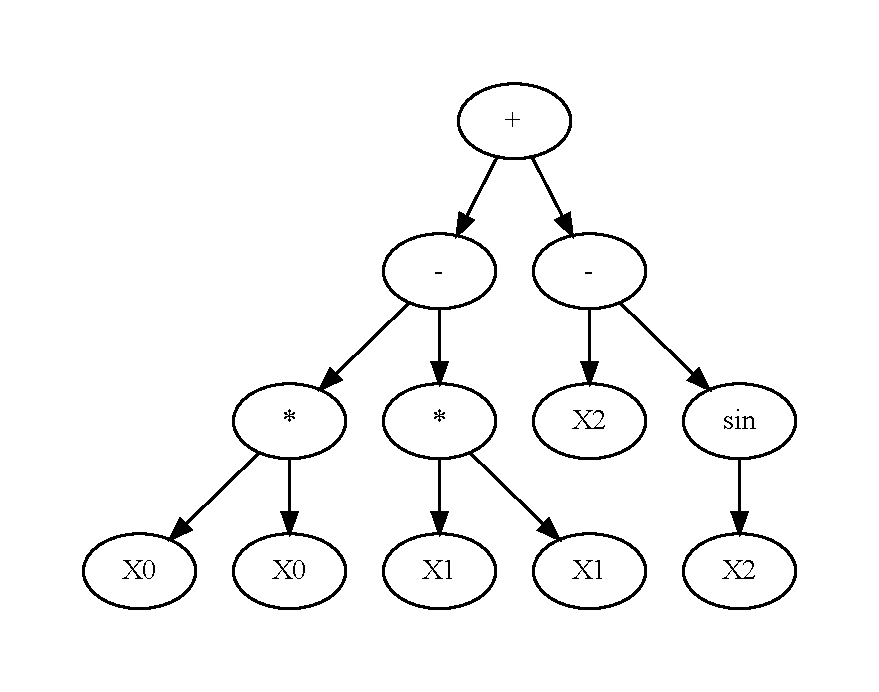
\includegraphics[scale=0.8]{images/graphviz/point_mut_before.dot.pdf}
    \caption{The original expression tree before performing a point mutation}
    \label{fig:point_muta}
  \end{subfigure}%
  \\
  \begin{subfigure}{\textwidth}
    \centering
    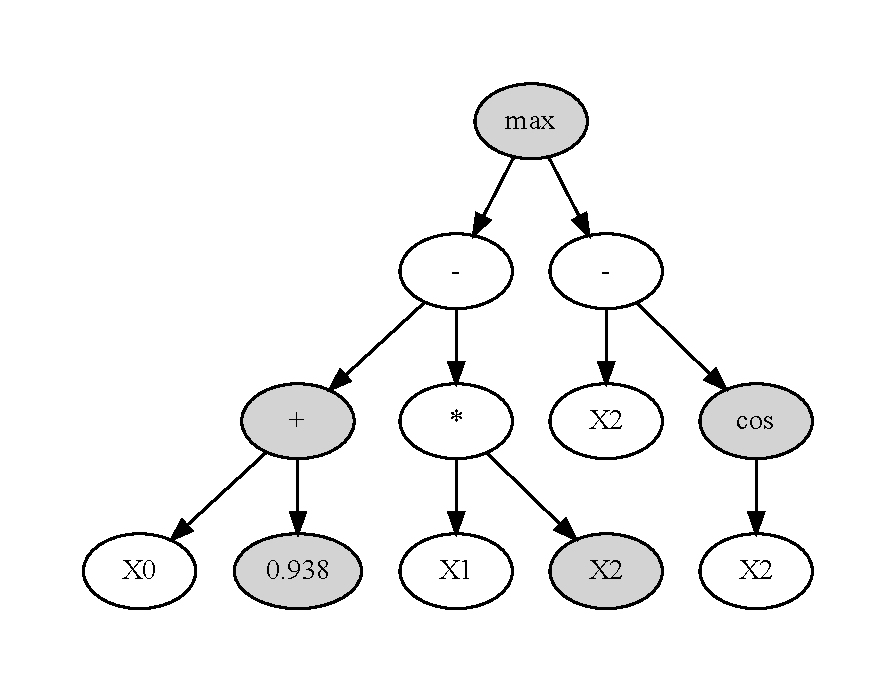
\includegraphics[scale=0.8]{images/graphviz/point_mut_after.dot.pdf}
    \caption{The same expression tree after a point mutation. The shaded nodes represent the changed terminals and functions in the final program.}
    \label{fig:point_mutb}
  \end{subfigure}
  \caption{Visualizing point mutations. Note that here, the program is the expression tree itself. }
  
  \label{fig:point}
\end{figure}

\subsubsection{Hoist Mutations}
\label{subsec:hoist}
In hoist mutations, we take the winner of a tournament and selects a random subtree from it. Another random subtree is selected from this subtree as a replacement for the subtree from the program. 

This mutation serves to reduce bloating of programs with increase in number of generations. \Cref{fig:hoist} visualizes the effect of hoist mutations on a given expression tree.

\begin{figure}[htp]
  \centering
  \begin{subfigure}{\textwidth}
    \centering
    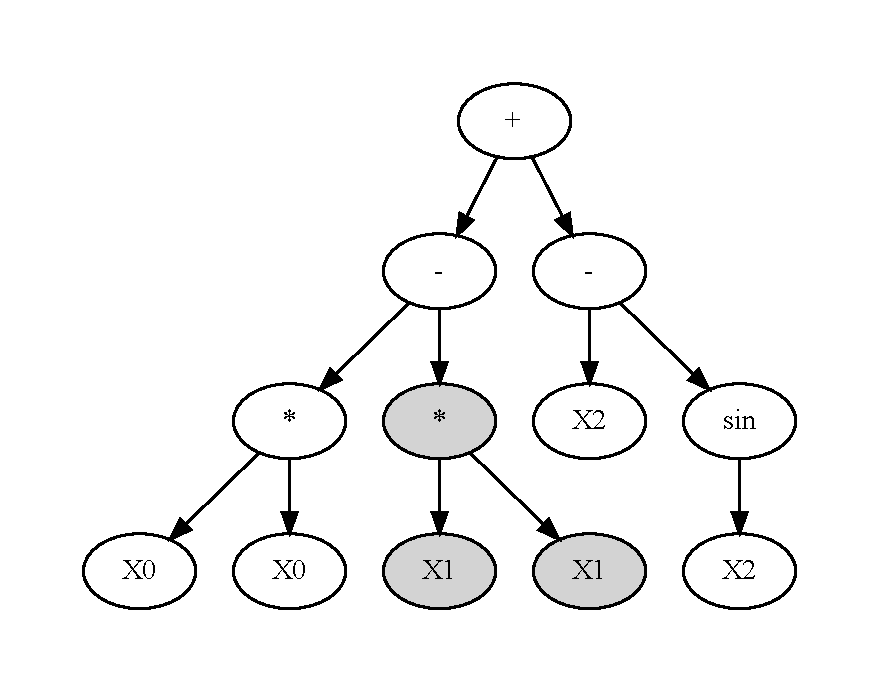
\includegraphics[scale=0.8]{images/graphviz/hoist_mut_before.dot.pdf}
    \caption{The original expression tree before performing a hoist mutation. The dark grey nodes denote the selected subtree, and the grey nodes denote the hoist subtree.}
    \label{fig:hoist_muta}
  \end{subfigure}%
  \\
  \begin{subfigure}{\textwidth}
    \centering
    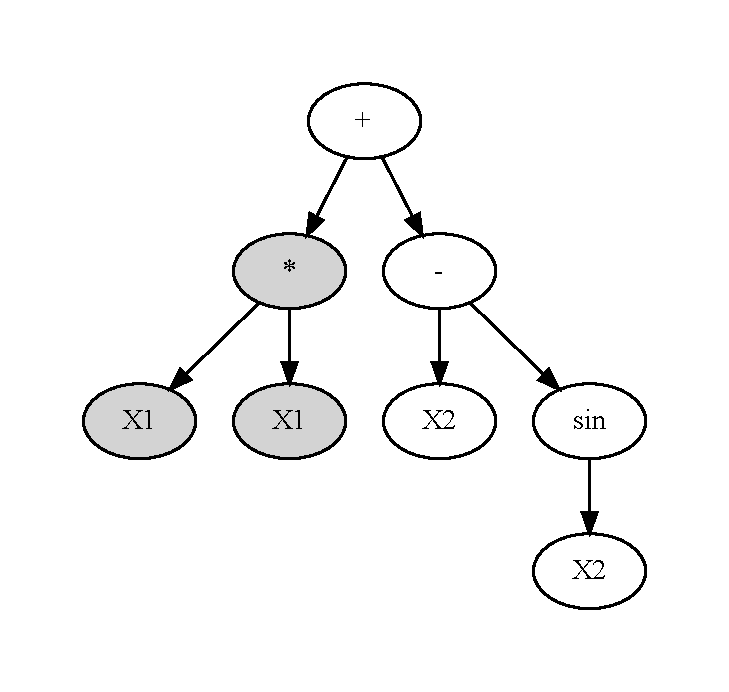
\includegraphics[scale=0.8]{images/graphviz/hoist_mut_after.dot.pdf}
    \caption{The same expression tree after hoisting the sub-subtree onto it's parent's position.}
    \label{fig:hoist_mutb}
  \end{subfigure}
  \caption{Visualizing hoist mutations for an expression tree. }
  
  \label{fig:hoist}
\end{figure}

\subsubsection{Crossover Mutations}
\label{subsec:crossover}
Crossover is a method of mixing genetic information between $2$ programs from a given population. In crossover mutations, we first determine a parent and a donor program using $2$ separate tournaments. We then select a random subtree of the parent program. The child program for the next generation is generated by replacing this subtree with a random subtree from the donor program. 

Crossover is considered as the principal method for evolution in our implementation, which is again inspired by \citep{gplearn}. We show a sample visualization of the crossover operation in \Cref{fig:crossover}.

\begin{figure}[htp]
  \centering
    \begin{subfigure}{\columnwidth}
      \begin{adjustbox}{width=\columnwidth,center}
        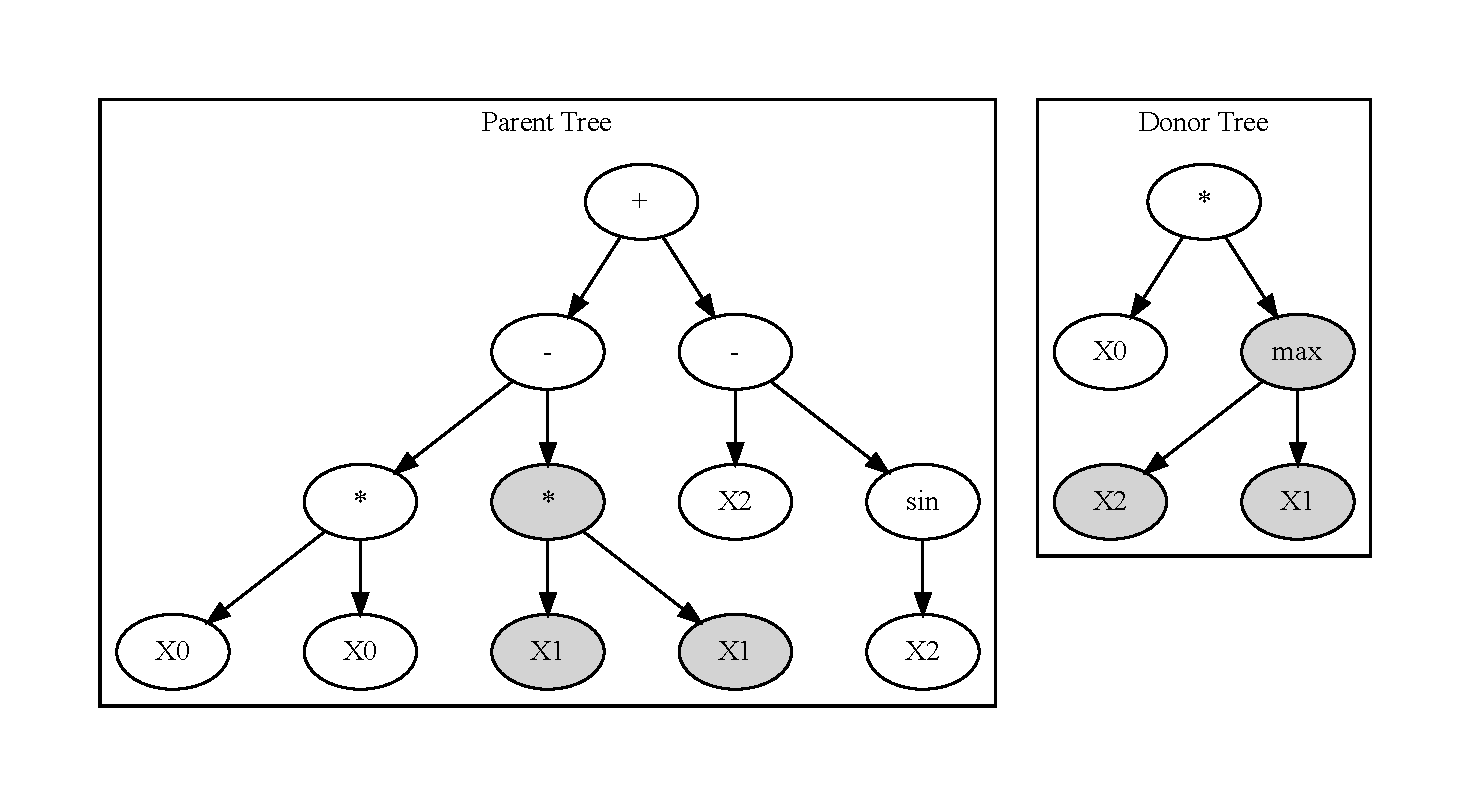
\includegraphics{images/graphviz/crossover_before.dot.pdf}
      \end{adjustbox}
      \caption{The parent and donor expression trees, both selected through tournaments are shown here.}
      \label{fig:crossover_muta}
    \end{subfigure}%
    \\
    \begin{subfigure}{\textwidth}
      \centering
      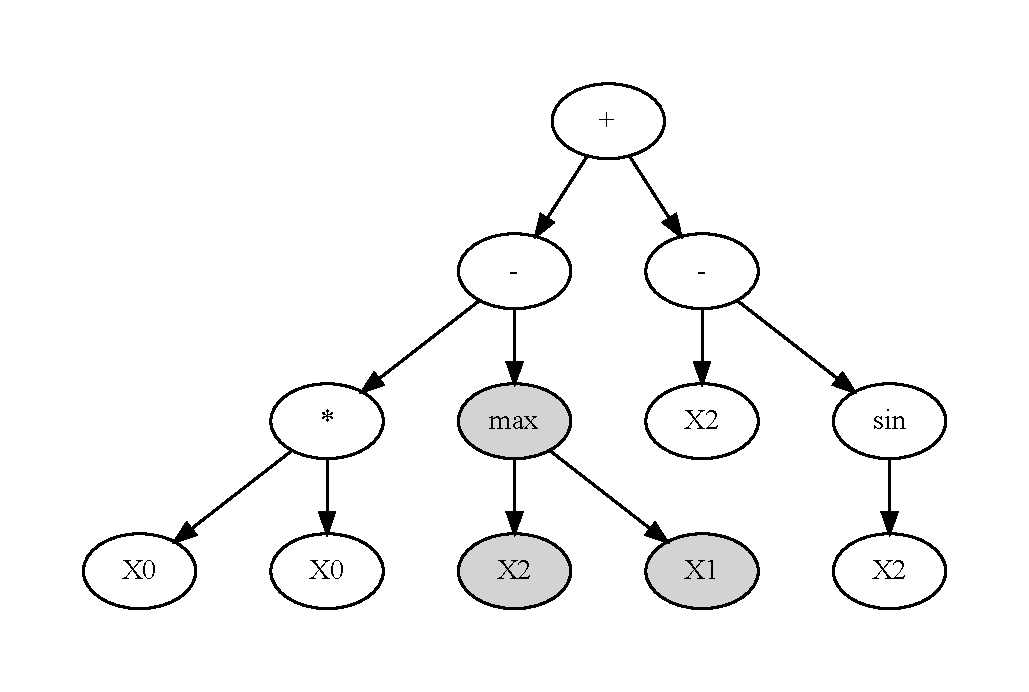
\includegraphics[scale=0.75]{images/graphviz/crossover_after.dot.pdf}
      \caption{The child expression tree after replacing a subtree of the parent with that of the donor.}
      \label{fig:crossover_mutb}
    \end{subfigure}
  \caption{Visualizing crossover mutations for a given parent and donor program.}
  
  \label{fig:crossover}
\end{figure}

\subsubsection{Subtree Mutations}
\label{subsec:subtree}
In subtree mutations, we perform a crossover between the winning parent tree and a randomly generated program. It serves as a method to increase new terminals and extinct functions in the next generation of programs, and is more aggressive compared to a crossover mutation\citep{gplearn}.

\Cref{fig:subtree} visualizes a sample subtree mutation in practice. We note that it is almost the same as the crossover visualization in \Cref{fig:crossover}, with  the exception being that the donor tree in \Cref{fig:crossover_muta} is now a randomly generated tree in \Cref{fig:subtree_muta}. 

\begin{figure}[htp]
  \centering
  \begin{subfigure}{\textwidth}
    \begin{adjustbox}{width=\columnwidth,center}
      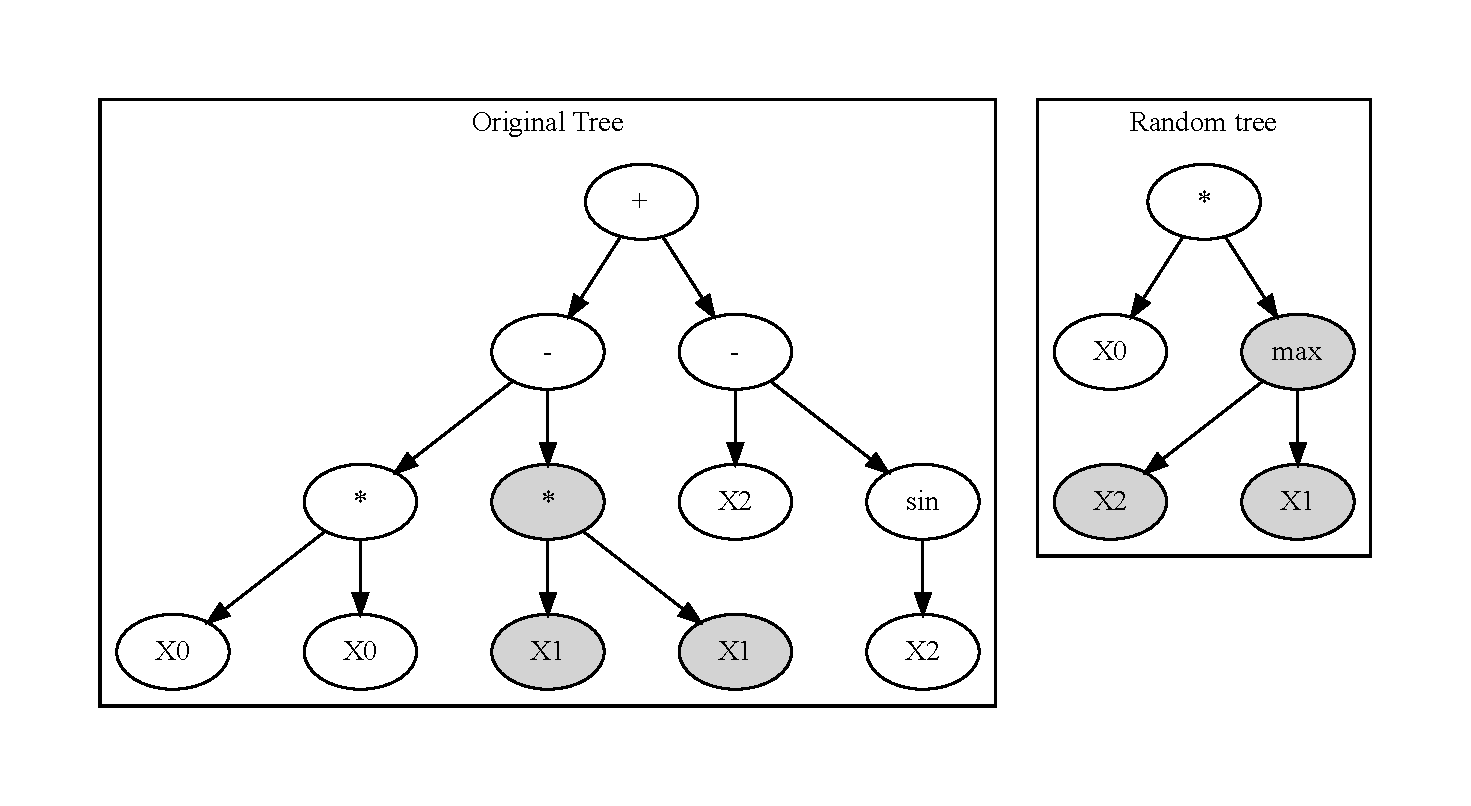
\includegraphics{images/graphviz/subtree_before.dot.pdf}
    \end{adjustbox}
    \caption{The parent expression tree and a randomly generated tree is shown here.}
    \label{fig:subtree_muta}
  \end{subfigure}%
  \\
  \begin{subfigure}{\textwidth}
    \centering
    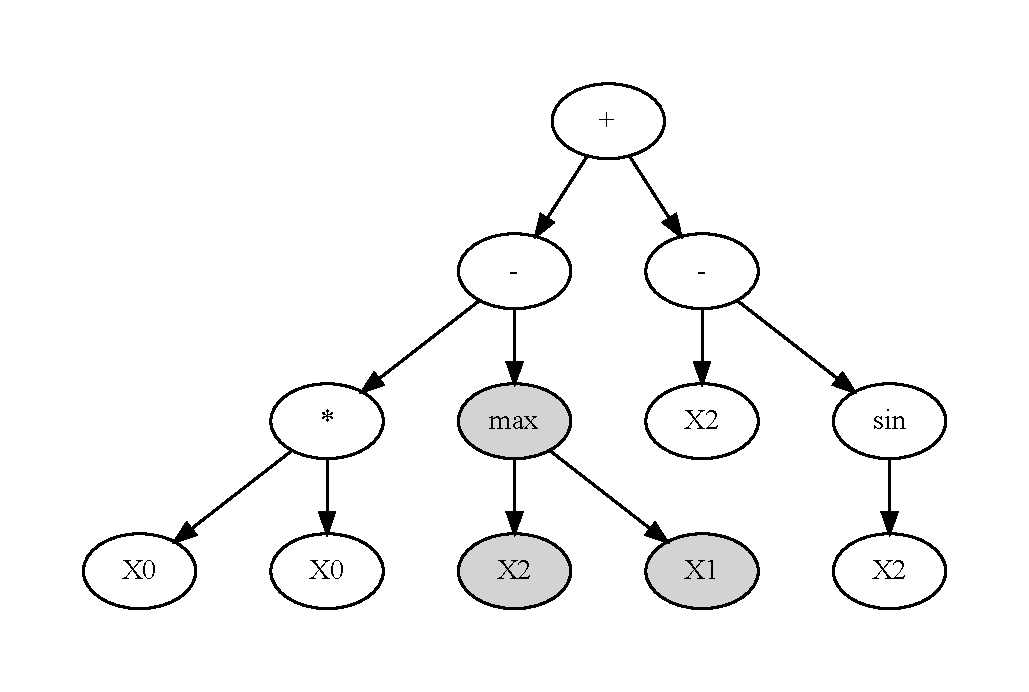
\includegraphics[scale=0.75]{images/graphviz/subtree_after.dot.pdf}
    \caption{The child expression tree after replacing a subtree of the parent with that of the random tree.}
    \label{fig:subtree_mutb}
  \end{subfigure}
  \caption{Visualizing subtree mutations for a given parent program.}
  \label{fig:subtree}
\end{figure}
  
\subsection{Evaluation}
\label{subsec:evaluation}
Once the population for the next generation is decided after selection and mutation, the fitness of all programs in the new generation is recomputed. This step is the major bottleneck when scaling the generational GP algorithm to bigger datasets and bigger populations, as the evaluation is independent for every program and every row of the input dataset. 

We perform the evaluation and computation of fitness in our implementation using a CUDA kernel and linear algebra primitives specified in the RAFT library(\citep{raschka2020machine}).

\section{Existing Libraries and Their Coverage}
\label{sec:otherlibs}
The table below(mostly reproduced from \cite{baeta2021speed}) lists some common libraries  used for genetic programming.  

\begin{table}[htbp]
  \caption{Existing GP frameworks along with language and device support}
  \begin{center}
      \begin{tabular}[c]{ccc}
          \toprule
          \textbf{Framework} &   \textbf{Language} & \textbf{Compute Type} \\
          \midrule
          KarooGP & Python & CPU/GPU \\
          TensorGP & Python & CPU/GPU \\
          DEAP & Python & CPU \\
          gplearn  & Python & CPU \\
          ECJ & Java & CPU \\
          \bottomrule
      \end{tabular}
      \label{tab:otherlibs}
  \end{center}
\end{table}

Among the libraries listed in \Cref{tab:otherlibs}, both TensorGP\citep{baeta2021tensorgp} and KarooGP\citep{staats2017tensorflow} use the TensorFlow python framework to perform fitness evaluation the GPU. However, while KarooGP uses TensorFlow's \textit{graph} execution model, where every program is compiled into an optimized computation DAG, TensorGP uses TensorFlow's \textit{eager} execution model\citep{agrawal2019tensorflow}, where expressions are evaluated immediately without the overhead of graph construction. The GPU parallelization here is through the use of TensorFlow-based vectorization, and not the explicit use of CUDA. 

DEAP\citep{DEAP_JMLR2012} is another commonly used Evolutionary Computing framework in Python implements a parallelized version of the GP framework. However, it offers only CPU based parallelization. 

Gplearn\citep{gplearn} is another Python framework which provides a method to build GP models for symbolic regression, classification and transformation using an API which is compatible with scikit-learn\citep{scikit-learn}. It also provides support for running the evolutionary process in parallel. The base code that is parallelized on GPUs in this thesis is largely inspired by gplearn. 

The ECJ Evolutionary Computing Toolkit\citep{Luke1998ECJSoftware} is a Java library for many popular EC algorithms, with an emphasis towards genetic programming. Almost all aspects of \Cref{gpalgo} are governed by a hierarchy of user-provided parameter files and classes, and the framework itself is designed for large, heavyweight experimental needs. Using ECJ parameter files, it is also possible to define custom GP pipelines with user-defined evolution strategies.

In the next chapter, we will talk about our work on parallelizing the GP algorithm to perform symbolic regression.
\chapter{OUR PARALLEL GP MODEL}
\label{chap:ourwork}
This chapter contains the implementation details of our parallel algorithm to perform genetic programming using CUDA. We first talk about a way to represent programs on the GPU. This is then followed by a description of the device side data structures used. We then give an overview of our modified GP algorithm, describing GPU-side optimizations for the selection, and evaluation step in detail. We also include details about the fitness computation step which comes after the evaluation step. Finally, we talk about the various challenges faced during the implementation of the modified algorithm, and the workarounds to avoid these problems.

In this implementation, we use a fixed list of functions with a maximum arity of $2$. We also assume that the maximum depth of all expression trees is a constant. This assumption is needed in order to evaluate the trees in the GPU using a fixed size stack.

\section{Program Representation}
\label{ow:input}
We define a struct for a program containing the following components. 
\begin{itemize}
    \item An array of operators and operands of the underlying expression tree stored in Polish(prefix) notation.
    \item A length parameter corresponding to the total number of nodes in the expression tree. 
    \item A raw fitness parameter containing the score of the current tree on the input data-set. 
    \item The depth of the current expression tree. 
\end{itemize}

\Cref{lst:programstruct} shows the internal definition of the program struct used in our code. \lstinline!nodes! here is the prefix list used to store the nodes of the underlying AST. The content of \lstinline!nodes! is decided through the mutation step. Evaluation and fitness computations are used for the computation of the \lstinline!raw_fitness_! field.

\begin{lstlisting}[caption={Our code for the program struct, representing a single expression tree. This entire structure is copied over and evaluated on the GPU.},label={lst:programstruct}]
struct program {
  explicit program();
  ~program();
  explicit program(const program &src);
  program &operator=(const program &src);

  node *nodes;
  /** total number of nodes in this AST */
  int len;
  /** maximum depth of this AST */
  int depth;
  /** fitness score of current AST */
  float raw_fitness_;
  /** fitness metric used for current AST*/
  metric_t metric;
  /** mutation type responsible for production */
  mutation_t mut_type;
};  // struct program
\end{lstlisting}

The entire population for a given generation is thus stored in an Array of Structures(AoS) format. The evaluation using a stack is almost similar to the way the Push3 system \citep{push3Stack} evaluates GP programs, with the sole exception being the reverse iteration due to the prefix notation chosen for the trees. 

Prefix notation was used for the representation of nodes to aid with the process of generating random programs, where we directly generate a valid prefix tree on the CPU.

\subsection{Device Side Data Structures}
\label{ow:deviceds}
In order to perform tournament selection and evaluation on the GPU, we use the following device side data-structures. 
\begin{itemize}
    \item \textbf{Philox Random Number Generator(RNG)} - We use a Philox counter-based RNG\citep{Philox2011} implemented in the {\bf raft} library\citep{raschka2020machine} to generate random global indices for tournament selection inside the selection kernel. 
    \item \textbf{Fixed size device stack} - We define a fixed size stack using a custom class, implementing the \textit{push}, \textit{pop} methods as inline \lstinline!__host__ __device__! functions. To avoid global memory accesses and encourage register look-ups for internal stack slots, the push and pop operation is implemented using an unrolled loop over all the available slots. This action is possible because the maximum size of the stack is fixed at $20$ for now. We shall discuss more about this in \Cref{sec:challenges}, where we examine how to avoid thread divergence in this setup.
\end{itemize}

Our kernels for both selection and program execution have been written in a way to eliminate any need for thread or memory synchronization. 

\subsection{Memory Footprint}
\label{ow:memory}
We examine the memory footprint of our implementation with respect to the number of programs stored in both CPU and GPU memory below. 
\begin{itemize}
    \item \textbf{CPU} --- Depending on a user-specified flag, we maintain a history of all the programs for all generations. If this is not desired, then we only store information about $2$ generations, the current and the next generation until the end.
    \item \textbf{GPU} --- Only the device memory corresponding to the current and the next generation of programs is stored through the run of the algorithm. During the course of the algorithm, the $2$ memory locations are updated with new programs in a ping pong fashion.
\end{itemize}

We will now explain our code for implementing parallel GP in \Cref*{ow:paralgo}.
\section{The Parallel GP Algorithm}
\label{ow:paralgo}
In this section, we again outline the individual steps of \Cref{gpalgo}, defined in \Cref{bgrw:algo}. However, each step contains details specific to our implementation. In this implementation, the selection and evaluation step is performed on the GPU, whereas mutations are carried out on the CPU.

Before performing any of the standard steps, we decide on the type of mutation through which the next generation program is produced. This mutation type selection is governed by user defined probabilities for the various types of mutations. This step is important, as we need to determine the exact  number of selection tournaments to be run(as crossovers require $2$ tournaments to decide the parent and donor trees). 

Once exact number of tournaments has been decided, we move on to the selection step.

\subsection{Selection}
\label{ow:selection}
We perform selection by running parallel tournaments in a CUDA kernel. For a population of size $n$ and tournament subset size $k$, we launch a CUDA kernel with $\left\lfloor n/256 \right\rfloor $ blocks and $256$ threads. In each thread, we generate $k$ random program indices using a Philox RNG(see \cref{ow:deviceds}). 

The index of the best program among the $k$ indices (based on the raw fitness values of the device programs) is then chosen as the winning index for the given thread, and is recorded in a \lstinline!win_indices! array.

\subsection{Mutation}
\label{ow:mutation}
The mutation of programs takes place on the CPU itself. We implement all the mutations mentioned in \cref{subsec:mutation} with a slight modification to the crossover operation in order to constrain the depth of the output tree. We call this modification a hoisted crossover.  

\subsubsection{Hoisted Crossover}

In this mutation, we initially perform a crossover between the parent tree and the donor tree. The selected subtree of the donor is then repeatedly hoisted onto the parent tree until the depth of the resultant tree is less than the maximum evaluation stack size. \\
Note that the hoist mutation occurs only on the donor sub-tree, since that is the part of the tree which contributes to the depth violation. If this was not the case, then another sub-tree of the parent sub-tree would have contributed towards the max depth violation, making the parent program itself an invalid one. \\
This modification is necessary for our code since a stack of fixed size $m$ can only evaluate a tree of depth $m-1$(assuming the maximum function arity is $2$)

At the end of mutations, we allocate and transfer the newly created programs onto GPU memory, in order to evaluate them on the input data-set. In order to save on device memory, we also deallocate the GPU memory of the previous population trees. Some of the challenges we faced due to the nested nature of programs during the \lstinline!cudaMemcpy! operations between host and device memory are listed in \Cref{sec:challenges}. 

\subsection{Evaluation}
\label{ow:evaluation}
We divide the evaluation portion into $2$ steps, namely execution and metric computation. In the execution step, all programs in the new population are evaluated on the given data-set, to produce a set of predictions. Once we have the predicted values for all programs, we compute the raw fitness value of the every program with respect to the expected output using the user-defined metric. These steps are explained in detail below.  

\subsubsection{Execution}
\label{subsec:execute}
For every program in the population and every sample in the input dataset, we produce predicted output values in this step. If $n$ is the population size, and $m$ is the number of samples in the input dataset, then we launch an execution kernel with a 2D grid of dimension $(\left\lceil m/256\right\rceil ,n)$ with $256$ threads per block. Each thread has its own device side stack which evaluates a program on a specific row.

We note here that to avoid thread divergence in the execution kernel, it is important to ensure that each block of threads execute on different rows of the same program. We provide more details about this in \Cref{sec:challenges}.

\subsubsection{Fitness Metric Computation}
\label{subsec:fitness}
In the previous step, after running the execution kernel, for all programs in the population, we have a list of predicted values. We also have access to the list of actual outputs. 

For every program, we compute fitness using a user-selected loss function. The inputs to the loss function are the program's output values(from the execution step) and the actual outputs.

Since the fitness computation is the same for all programs, we computed loss for all programs in parallel on the GPU. This was implemented using the matrix-vector linear algebra primitives present in the \textbf{raft} library\citep{raschka2020machine}, where the vector of actual output values is reused for all predicted values of different programs. We implement a weighted version of the following $6$ standard loss functions:
\begin{itemize}
    \item Mean Absolute Error (MAE)
    \item Mean Square Error (MSE)
    \item Root Mean Square Error (RMSE)
    \item Logistic Loss(binary loss only)
    \item Karl Pearson's Correlation Coefficient
    \item Spearman's Rank Correlation Coefficient
\end{itemize}
During the implementation of Spearman Rank Correlation, we used the \textbf{thrust} library from Nvidia to generate ranks for the given values. The default fitness function is set as MAE, in an effort to be consistent with gplearn\citep{gplearn}.

\section{Challenges Faced}
\label{sec:challenges}
In this section, we briefly talk about some challenges faced during the implementation of our parallel GP algorithm.

\subsection{Thread divergence and Global Memory Access}
\label{prob:divergence}
In the execution kernel, during the evaluation phase, when evaluating a stack node, we check for equality of the current function with $33$ pre-defined functions, using \lstinline!if-else! conditions on the node type. 

Since CUDA executes statements using warps of $32$ threads in parallel, when it encounters an \lstinline!if-else! block inside a kernel which is triggered only for a subset of the warp, both the \lstinline!if! and \lstinline!else! block are executed by all threads. During the execution of the \lstinline!if! block, the threads which don't trigger the \lstinline!if! condition are masked, but still consume resources, with the same behaviour exhibited for the \lstinline!else! block. This increases the total execution time as both blocks are effectively processed by all warp threads. 

To avoid this behaviour in our code, we ensure that within every thread-block of the execution kernel, all threads execute the same program. This ensures that all threads in a warp will always take the same branch during node identification, and thus avoid divergence during a single stack evaluation.

In the implementation of \textbf{push} and \textbf{pop} operations for the device side stack, we avoid trying a possible dereference using global memory index(the current number of elements in the stack) by using an unrolled loop for stack memory access. This is again safe from thread divergence because we ensure that within a thread-block, all threads evaluate the same program. 

\subsection{Memory Transfers and Allocation}
\label{prob:memcpy}
Since we went with a AoS representation for the list of programs and each program has a nested pointer for the list of nodes in it, we are forced to perform at least $2$ \lstinline!cudaMemcpy! operations per program in a loop spanning the population size. One of the copy operations is for the list of program nodes, and the other copy is to capture the metadata about the nodes, and the other copy is for the program struct itself. 

Since all our computations are ordered on a single CUDA stream, transferring programs back and forth the device in a loop slows down the overall time for training. However, in our experiments, we observed that the dominant contributor to execution time was the evaluation step, and not memory transfers. Thus, the implementation was not altered.

In the next chapter, we will describe some benchmark experiments and present our results. 

\chapter{Experimental Evaluation}
\chapter{SUMMARY AND FUTURE WORK}
\label{chap:conclusion}
In this chapter, we summarize some experimental results of \Cref{chap:experiments}, as well as provide an outline for further improvements, both with respect to optimizations and new features.

\section{Summary of Results}
\label{sec:summary}
In this work, we attempt to accelerate genetic programming based algorithms, for symbolic regression and transformation on the GPU. We do this by parallelizing the selection and evaluation step of the generational GP algorithm. We introduce a prefix-list representation for expression trees, which are then evaluated using an optimized stack on the GPU. Fully vectorized routines for standard loss functions are also provided, which can be used as fitness functions during the training of a genetic population of programs. At the end of a run, our algorithm returns the entire set of evolved programs for all generations. One can filter the most optimal program from the last generation of programs, or the programs with maximum variation (based on fitness values) to perform symbolic regression or transformation respectively. 

On synthetic datasets for the Pagie Polynomial ranging in size from $4096$ to $4$ million points, we were able to achieve an average speedup of $27\times$ with respect to gplearn\citep{gplearn}, a library our implementation takes inspiration from. Our algorithm evolves a set of $50$ programs for $50$ generations on a $4$ million rows in less than $10$ seconds. 
% Even the secret Joestar technique can't compare to this lol

\section{Further Improvements}
\label{sec:improvements}
In this section, we list out a few possible feature improvements and optimizations to our algorithm's implementation.

\subsection{Possible Optimizations}
\label{subsec:optimizations}
In our experiments, we found that for large datasets, maximum amount of GPU time (around $71.5\%$) is spent in the evaluation kernel. However, this was an expected figure, as evaluation is the main bottleneck for many GP programs. 

We note that as long as an exact copy of the population program exists, it doesn't matter if the representation of the program slightly changes on the device. Keeping this in mind, one can attempt to reduce the average depth of the trees being evaluated by performing some balancing on the device trees(while still maintaining the prefix order for all expressions). This will help in the evaluation step, as lesser stack slots will be used for a small-depth balanced tree compared to a larger depth unbalanced tree, leading to lower kernel stack memory usage per thread. However, we note that implementing tree balancing in the GPU is a non-trivial task.

Note that another optimization approach is to convert the current prefix-list into a DAG to cache values of common sub-expressions. However, in this case, the evaluation method of the underlying tree itself changes. 

\subsection{New Features}
\label{subsec:newfeatures}

Our implementation of genetic programming in cuML lacks a few features compared to other standard GP libraries. We discuss a few of these missing features, along with possible implementation strategies in the current scheme. 

\subsubsection{Supporting custom function sets}
Our current implementation of genetic programming in cuML provides a constant list of $33$ functions. We don't expose any way for users to define their own custom functions for use during evolution. 

Support for this can be added through the use of \lstinline!__host__ __device__! function pointers. The user can specify a list of function pointers as training hyper parameters. During the stack execution phase, the specified function pointer is called at runtime for evaluation.

\subsubsection{Custom Loss functions}

Since CUDA supports \lstinline!__host__ __device__! Lambda functions, custom loss functions are easier to support compared to custom function sets. The user can specify the loss function for a single predicted label in a lambda function. Vectorization of this loss function over the program population and input dataset can be done in a CUDA kernel to which the lambda function is passed as input. 


% End content
% \appendix
 
\chapter{A SAMPLE APPENDIX}
 
Just put in text as you would into any chapter with sections and
whatnot.  Thats the end of it.

% \listofpapers

\begin{enumerate}  
	\item Authors....  \newblock
	Title...
	\newblock {\em Journal}, Volume,
	Page, (year).
\end{enumerate}  
\pagebreak
\begin{singlespace}
 \begin{small}
    \bibliography{refs}
 \end{small}
\end{singlespace}
  

\end{document}
